\chapter{Snímky dokumentace}

\section{Úvodní obrazovka}

\begin{figure}[H]
  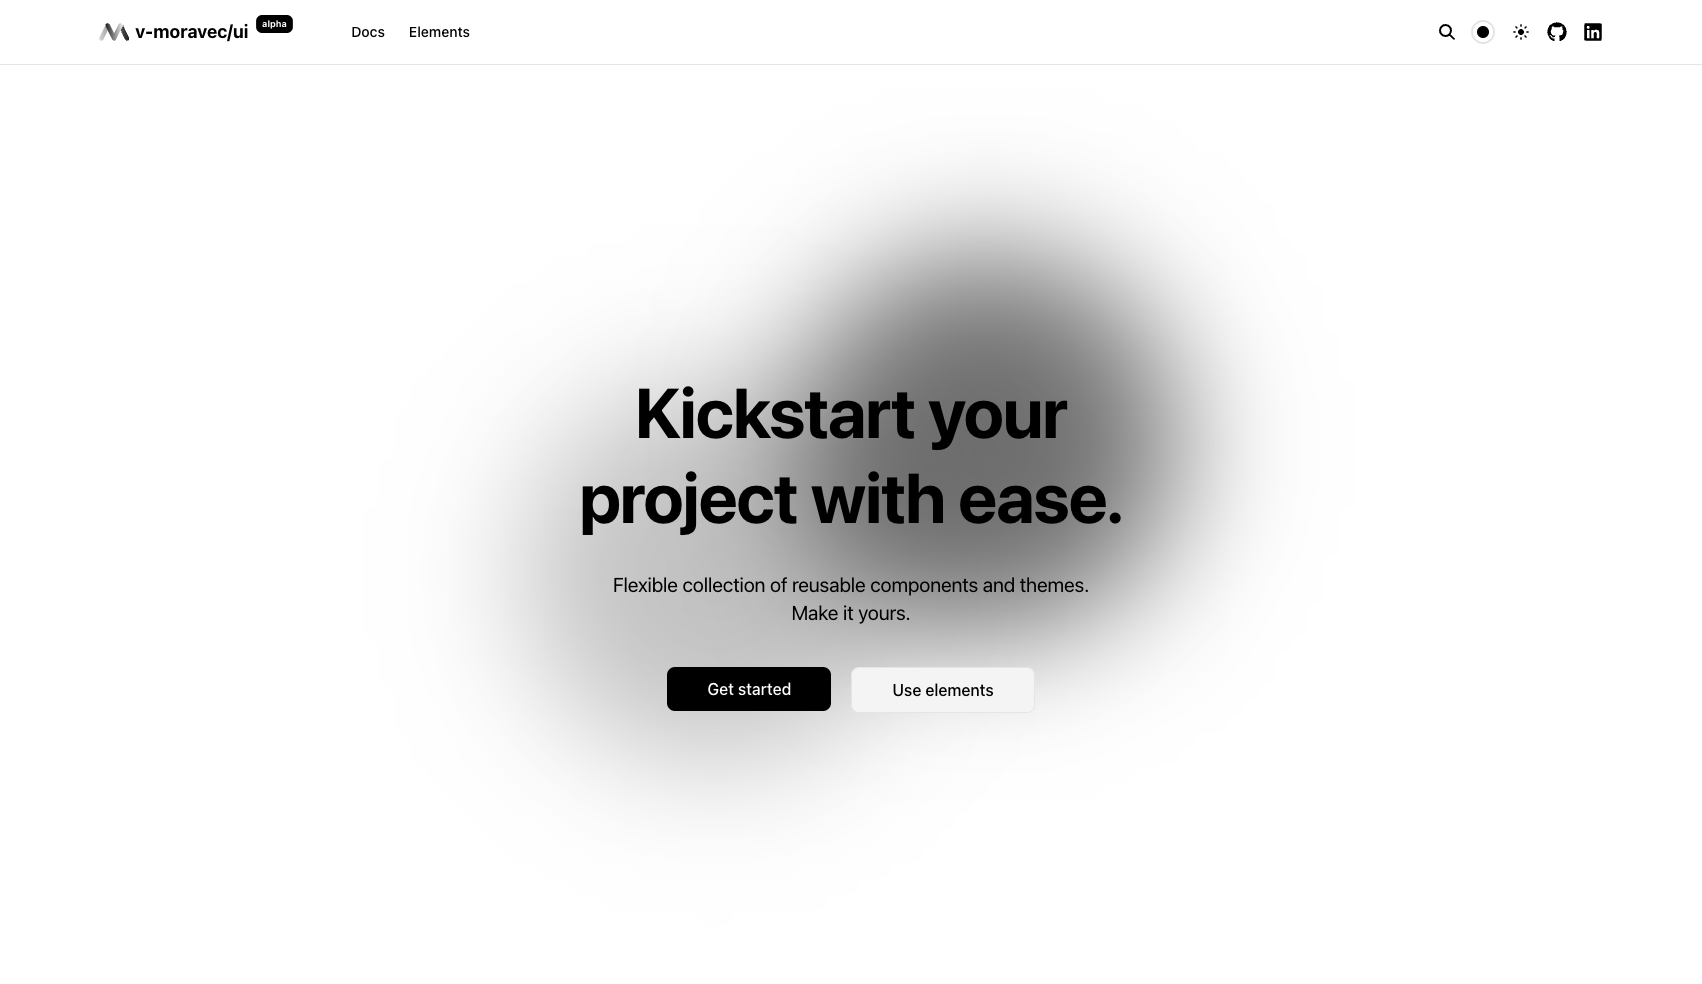
\includegraphics[width=\textwidth]{images/main-page}
  \caption{Úvodní obrazovka} \label{picture:documentation:main-page}
\end{figure}

\begin{figure}[H]
  \centering
  \subfloat[Tmavá verze]{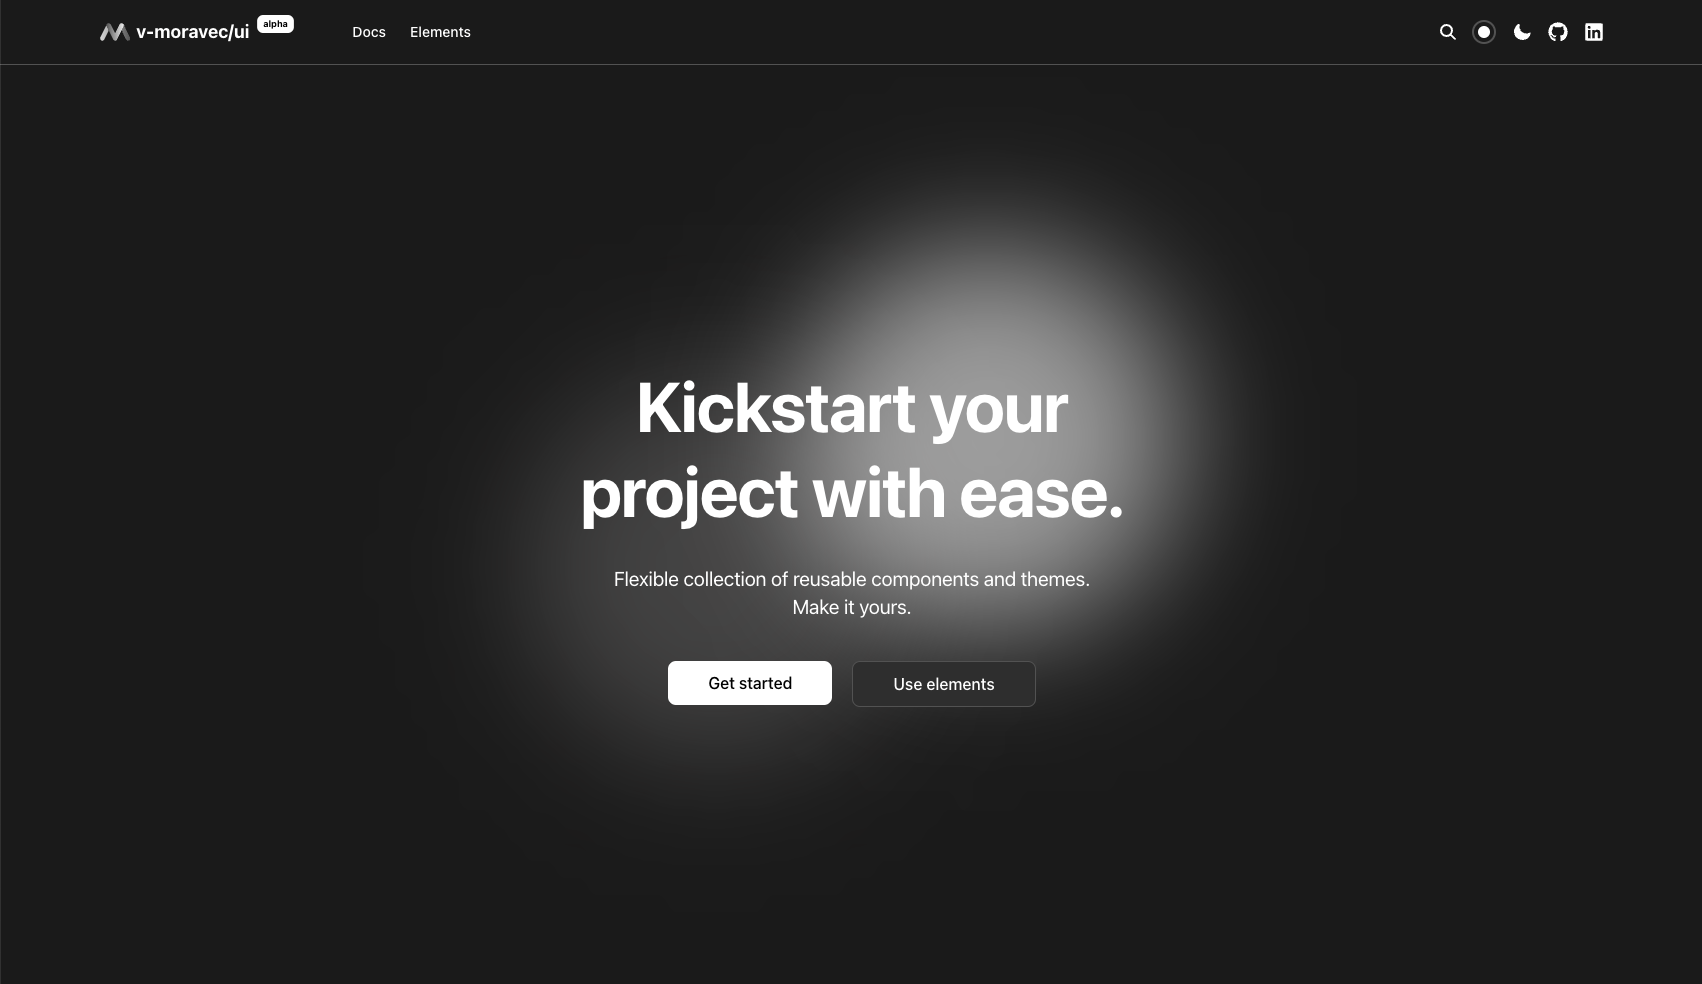
\includegraphics[width=0.3\textwidth]{images/main-page-dark}\label{picture:documentation:main-page-dark}}
  \subfloat[Modrá verze]{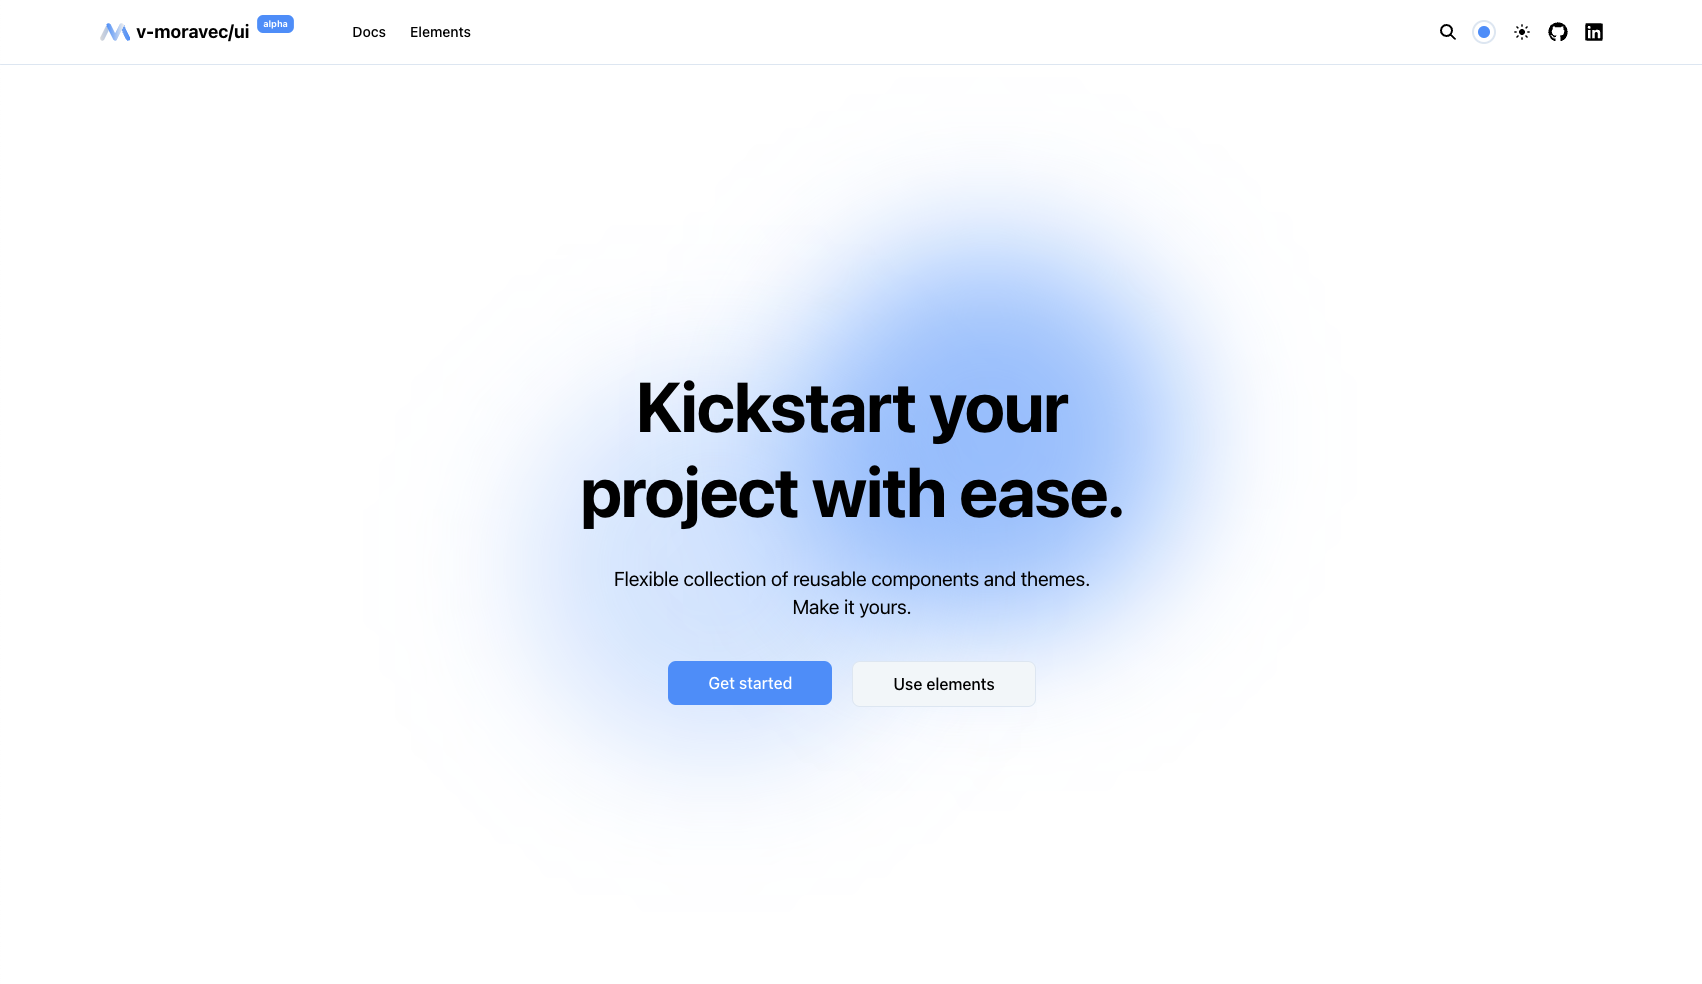
\includegraphics[width=0.3\textwidth]{images/main-page-colored}\label{picture:documentation:main-page-colored}}
  \caption{Stylování}
\end{figure}

\section{Komponenty}

\begin{figure}[H]
  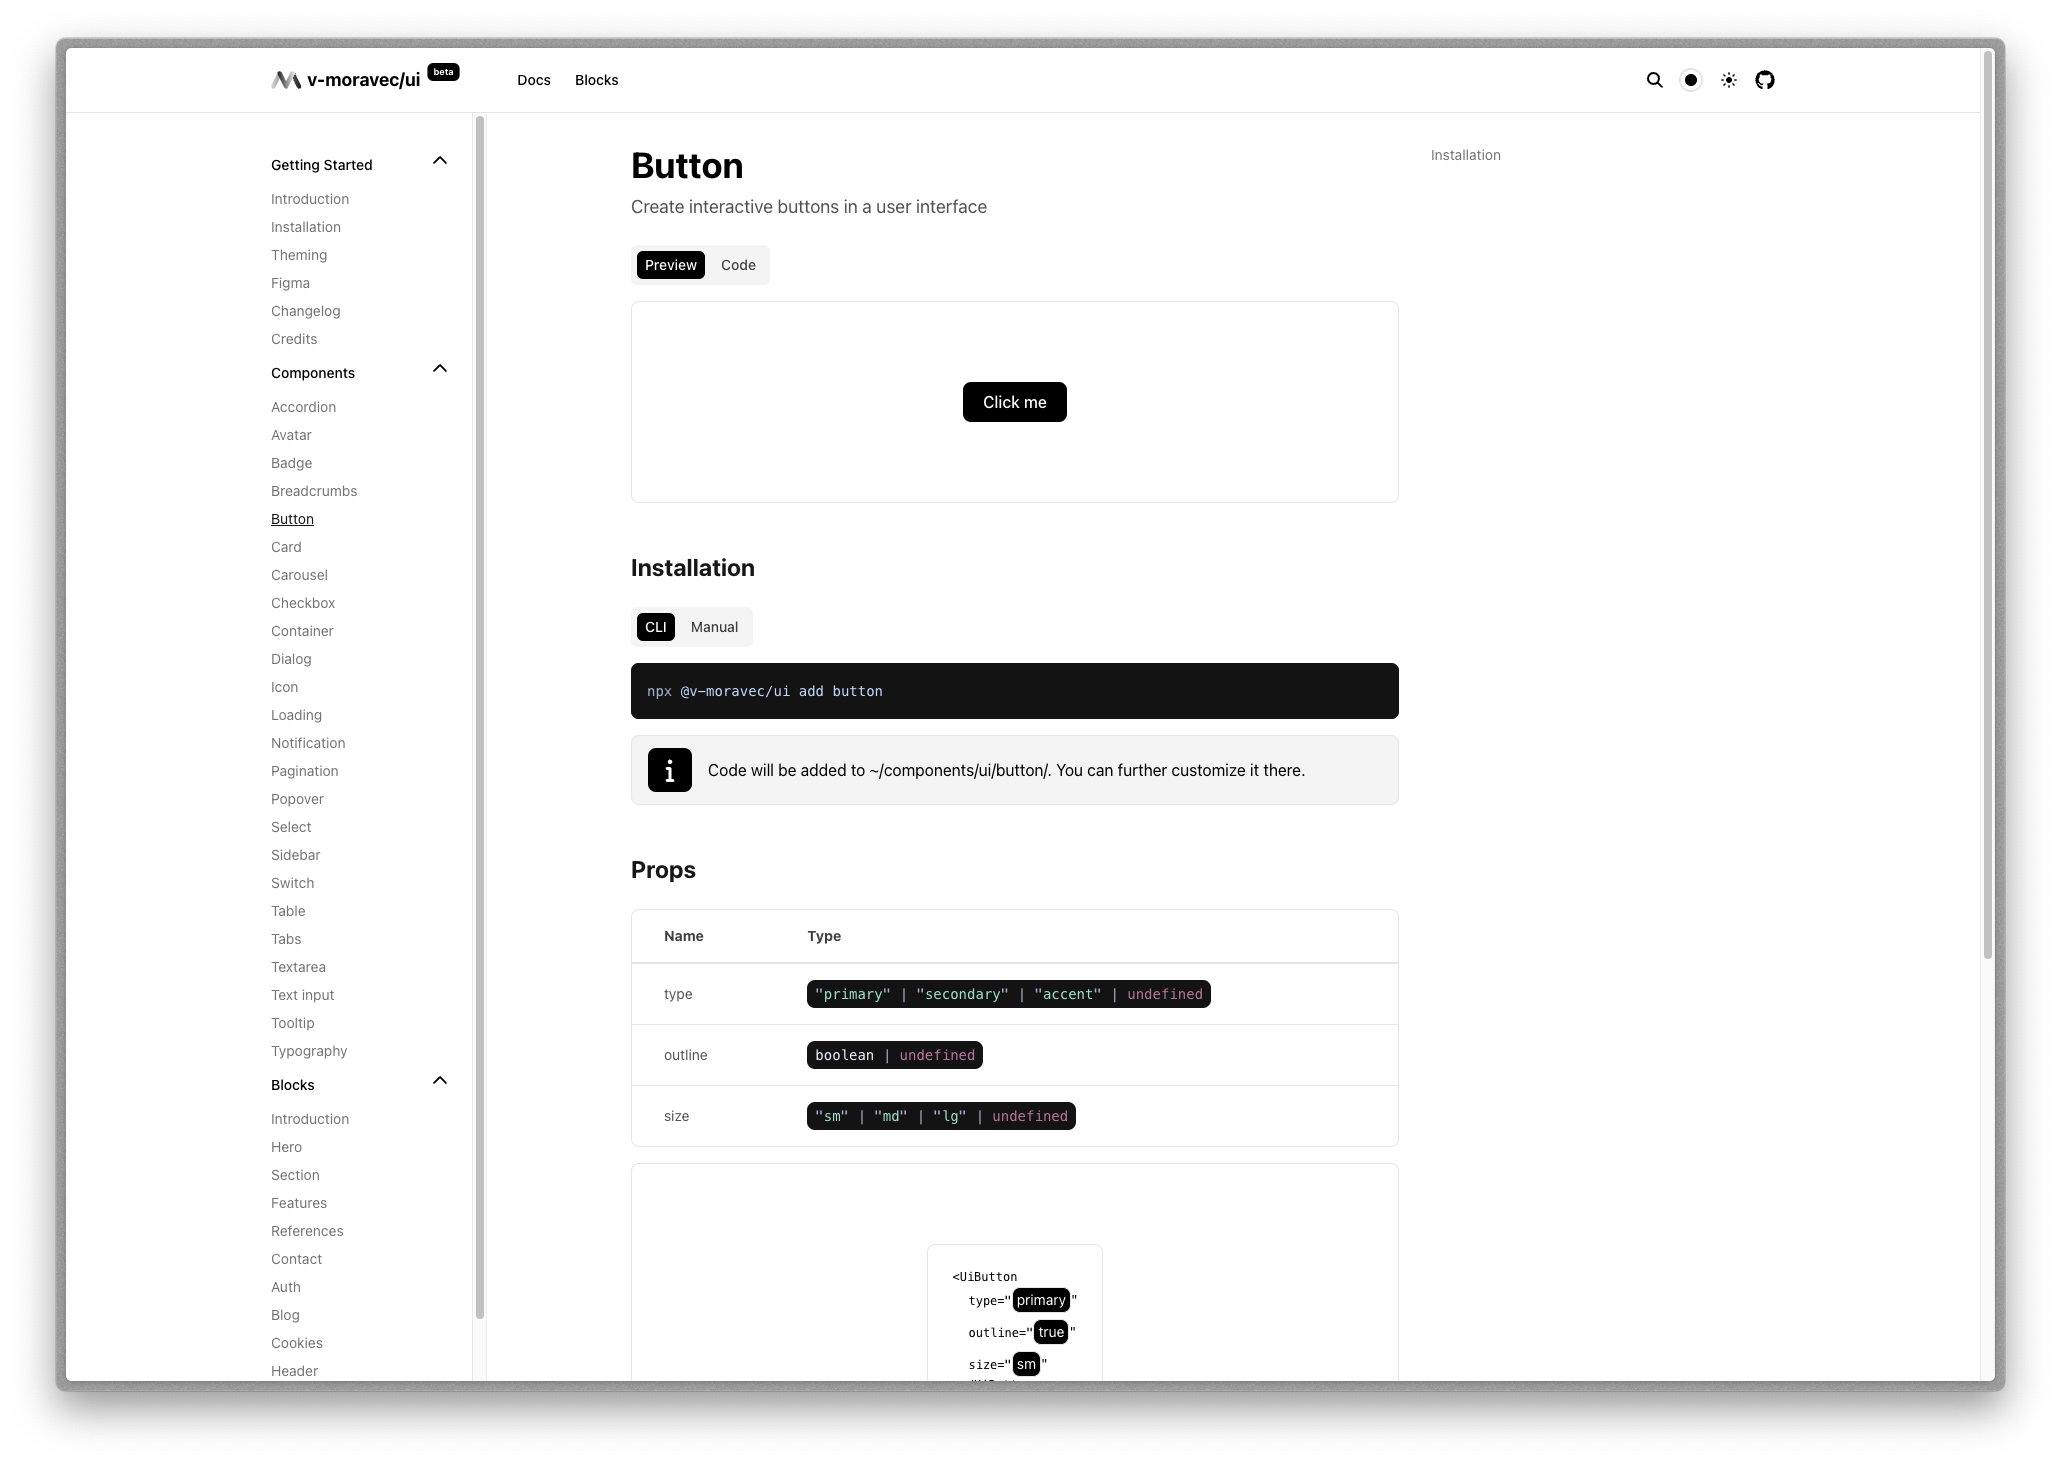
\includegraphics[width=\textwidth]{images/component-preview}
  \caption{Zobrazení komponenty} \label{picture:documentation:component-preview}
\end{figure}

\begin{figure}[H]
  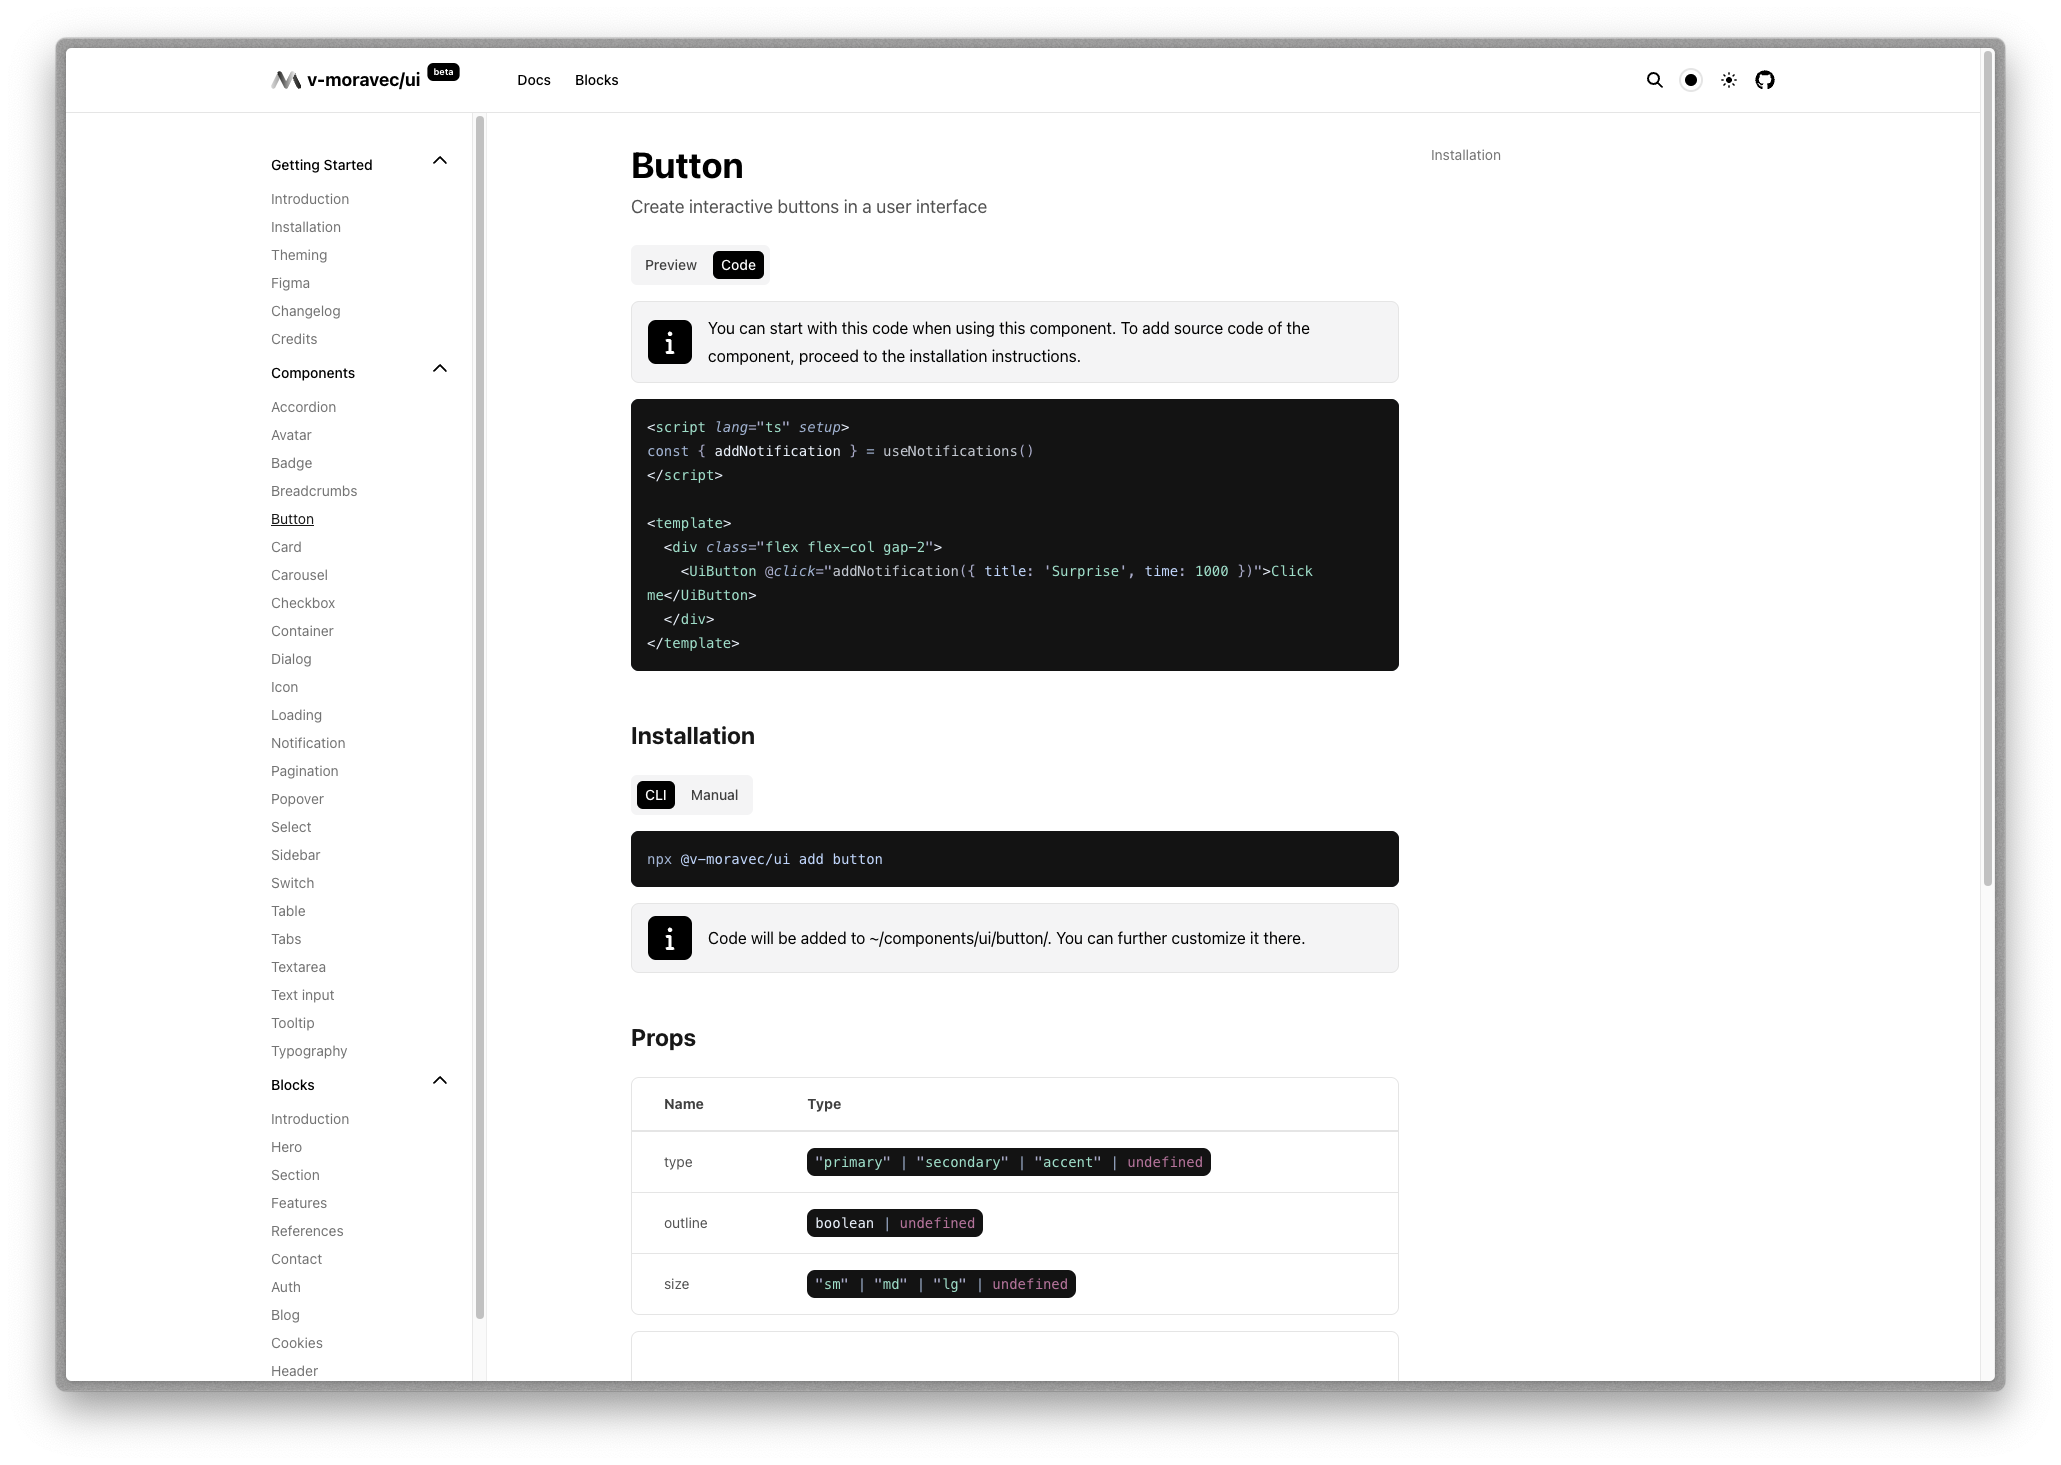
\includegraphics[width=\textwidth]{images/component-code}
  \caption{Kód komponenty} \label{picture:documentation:component-code}
\end{figure}

\section{Elementy}

\begin{figure}[H]
  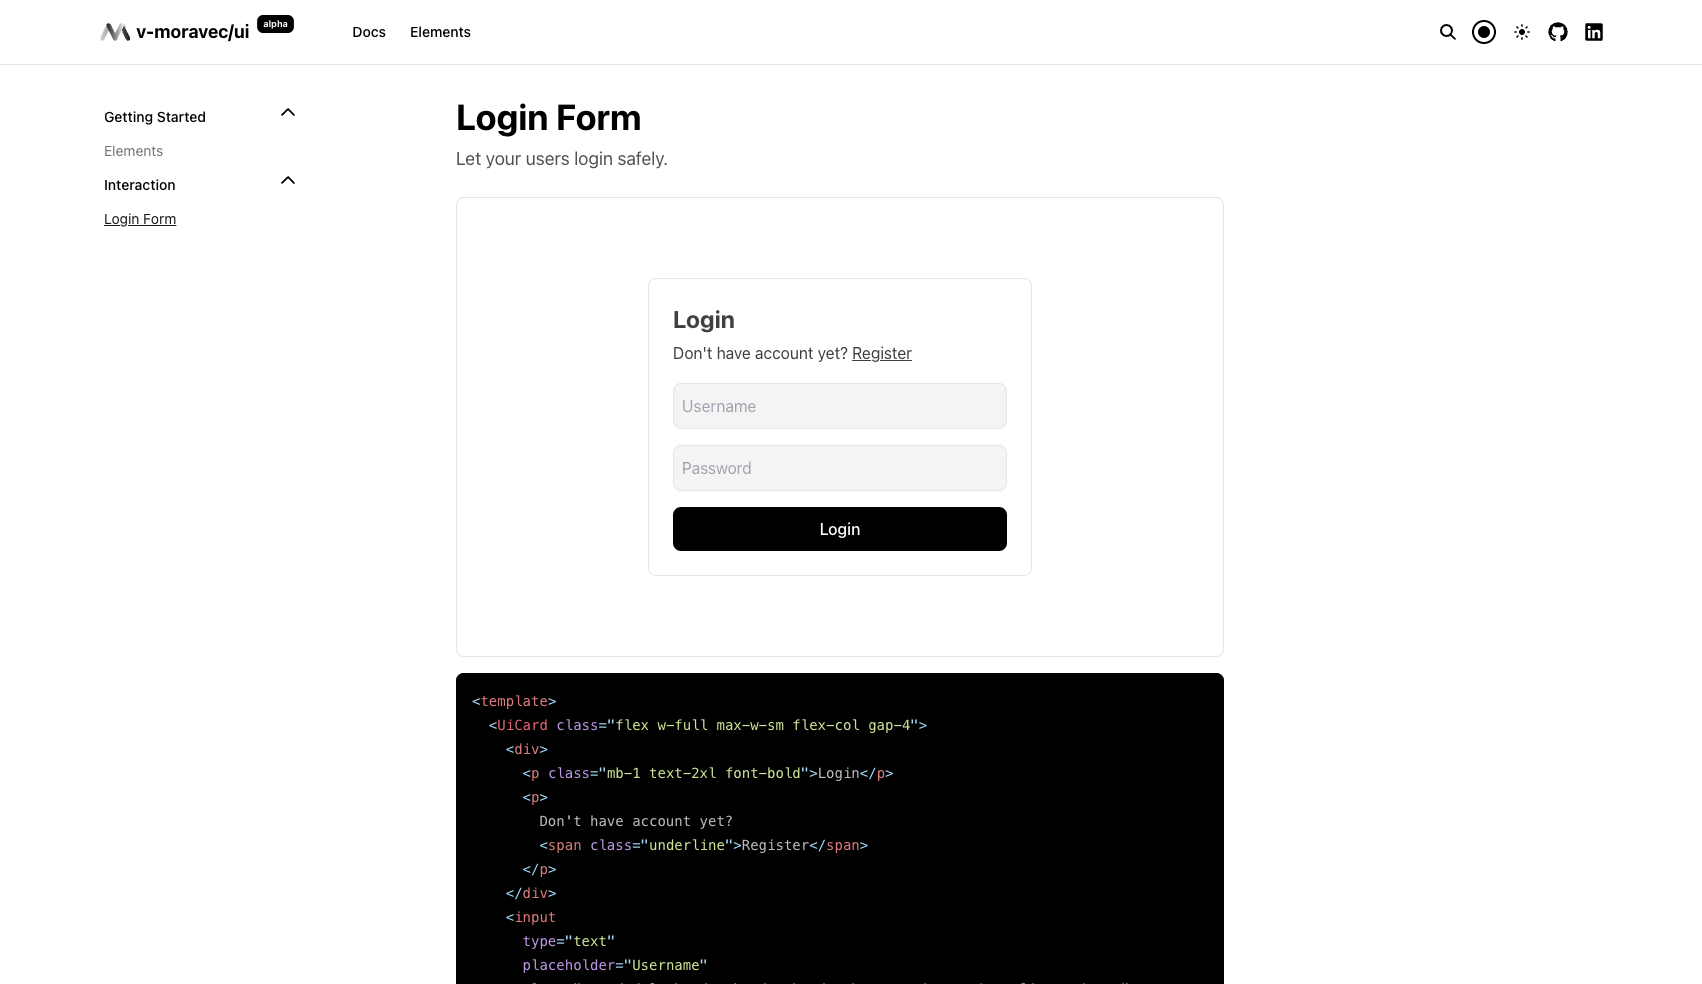
\includegraphics[width=\textwidth]{images/element}
  \caption{Element složený z komponent} \label{picture:documentation:element}
\end{figure}

\chapter{Ukázky kódu}

\begin{listing}[H]
  \caption{Vytvoření endpointu pro získání kódu komponent}
  \label{lst:link-to-endpoint}
  \begin{code}
nuxt.hook('nitro:config', (nitroConfig) => {
nitroConfig.virtual = nitroConfig.virtual || {}
  nitroConfig.virtual['#component-list/nitro'] = () =>
      readFileSync(join(nuxt.options.buildDir, '/component-list.mjs'), 'utf-8')
})

addServerHandler({
  method: 'get',
  route: '/api/component-list/:component?',
  handler: resolver.resolve('../server/api/component-list.get'),
})
\end{code}
\end{listing}

\begin{listing}[H]
  \caption{Endpoint pro získání kódu komponent}
  \label{lst:code-example-endpoint}
  \begin{code}
import { defineEventHandler, createError, appendHeader } from 'h3'
import { pascalCase } from 'scule'
// @ts-expect-error
import components from '#code-examples/nitro'

export default defineEventHandler((event) => {
  appendHeader(event, 'Access-Control-Allow-Origin', '*')
  const componentName = (event.context.params['component?'] || '').replace(/\.json$/, '')
  if (componentName) {
    const component = components[pascalCase(componentName)]
    if (!component) {
      throw createError({
        statusMessage: 'Examples not found!',
        statusCode: 404,
      })
    }
    return component
  }
})  
\end{code}
\end{listing}

\begin{listing}[H]
  \caption{Transformace dat komponent a bloků pro využití v rámci CLI}
  \label{lst:cli-data-transform}
  \begin{code}
const code = await fsp.readFile(component.shortPath, 'utf-8')

const script = code.match(/<script[^]*?<\/script>/ms)?.[0]
const template = code.match(/<template[^]*?<\/template>/ms)?.[0]

const dependencies = script
  ? removeDuplicates(
      script
      .match(/import[^]*?from[^]*?['"]([^'"]+)['"]/gm)
      ?.map((dependency) => {
          return dependency.split('from')[1].trim().replace(/['";]/g, '')
      })
      .filter((v) => !v.startsWith('.') && !v.startsWith('~') && v !== 'vue' && v !== 'nuxt')
  )
  : undefined

const composableDependencies = script
  ? removeDuplicates(
      script
      .match(/use[a-zA-z]*?\(/gm)
      ?.map((dependency) => {
          return dependency.trim().replace(/['"();]/g, '')
      })
      .filter((v) => !v.startsWith('.') && !v.startsWith('~') && v !== 'vue' && v !== 'nuxt')
  )
  : undefined

const uiDependencies = template
  ? removeDuplicates(
      template.match(/<Ui[^>]+>/gm)?.map((v) =>
      v
          .slice(1, -1)
          .split(' ')[0]
          .trim()
          .split(/(?=[A-Z])/)[1]
          .toLowerCase()
      )
  )
  : undefined

components[component.pascalName] = {
  code,
  uiDependencies,
  dependencies,
  composableDependencies,
  shortPath: component.shortPath,
  pascalName: component.pascalName,
}
\end{code}
\end{listing}

\begin{listing}[H]
  \caption{Komponenta pro zvýraznění kódu}
  \label{lst:code-highlighter}
  \begin{code}[html]
<script lang="ts" setup>
import { transformContent } from '@nuxt/content/transformers'

const props = defineProps<{
  name: string
  class?: string
}>()

const data = await fetchCodeExample(props.name)

const hasCode = computed(() => data?.code)

const highlighter = await loadShiki()
const { data: ast } = await useAsyncData(`content-example-${props.name}-ast`, () =>
  transformContent('content:_markdown.md', `\`\`\`vue\n${data?.code ?? ''}\n\`\`\``, {
    markdown: {
      highlight: {
        highlighter,
        theme: {
          light: 'poimandres',
          default: 'poimandres',
          dark: 'poimandres',
        },
      },
    },
  })
)
</script>

<template>
  <div class="my-4" v-if="hasCode">
    <ContentRenderer :value="ast" class="[&>div>pre]:!mt-0 [&>div>pre]:overflow-auto [&>div>pre]:!rounded-t-none" />
  </div>
</template>
\end{code}
\end{listing}
